% Use ONE language version. Full-width figure in a two-column paper.
% Assumed final width: 7 inches (177.8 mm); body labels remain about 8.1 pt.
\begin{figure*}[t]
  \centering
  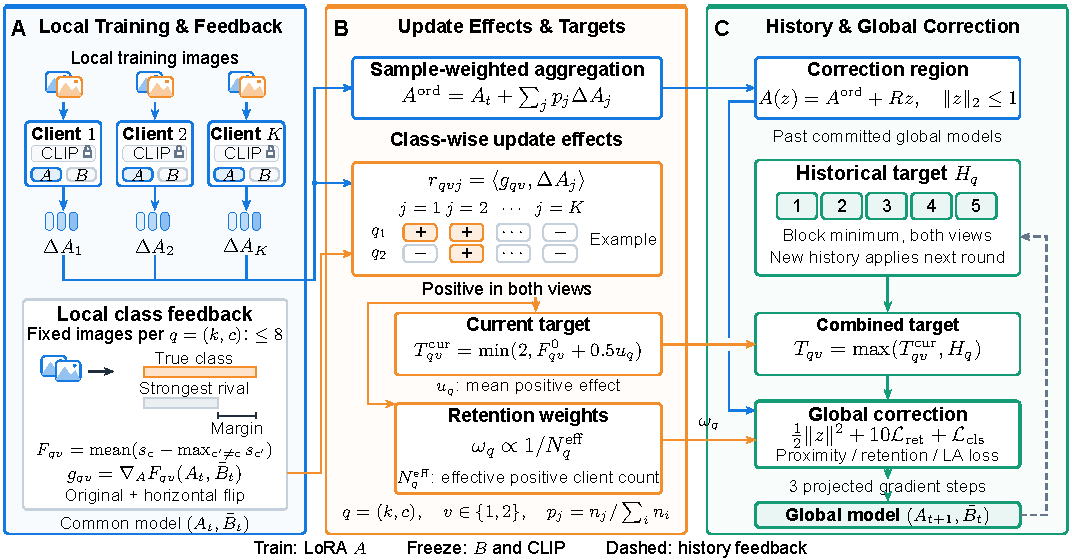
\includegraphics[width=\textwidth,keepaspectratio]{figures/tikz_method_a_overview_en.pdf}
  \caption{Overview of Method A. Client update effects determine current targets
  and margin-retention weights, while historical targets retain sustained
  improvements measured on fixed local training images. Ordinary aggregation
  keeps sample-size weights; the aggregate is then corrected in three projected
  steps. Icons, score bars, and response signs are schematic.}
  \label{fig:method-a-overview}
\end{figure*}

% Chinese version, to be used instead of the block above:
% 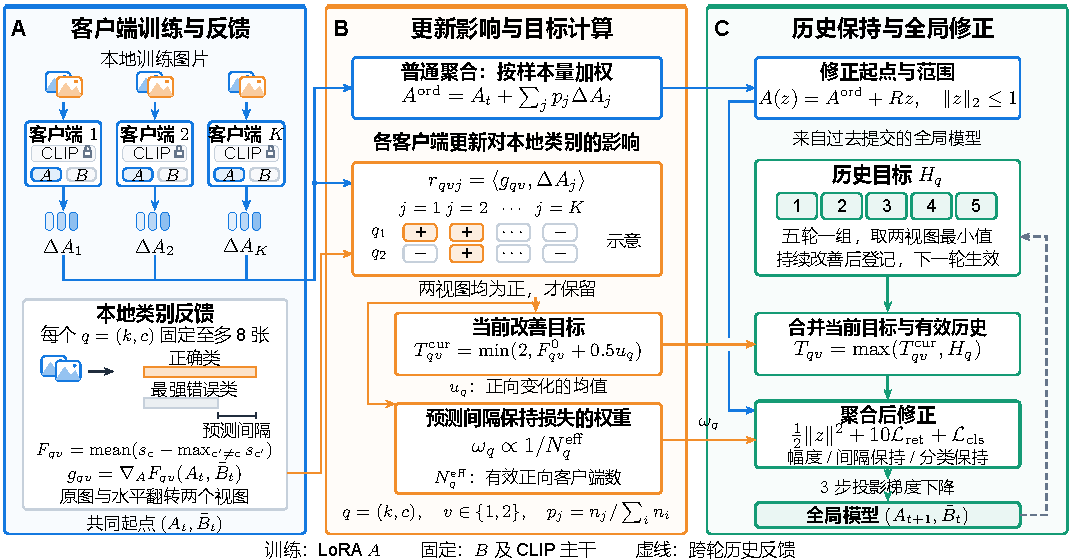
\includegraphics[width=\textwidth,keepaspectratio]{figures/tikz_method_a_overview_zh.pdf}
